\section{Datenbankdesign}
Um die Erweiterung der Datenbank für den Feasibility Check zu erklären, wird zunächst auf die grundlegende Struktur der REALIS-Datenbank eingegangen. In Abbildung \ref{fig:realis-datenbankdesign} ist ein Ausschnitt der wichtigsten Tabellen und deren Beziehungen dargestellt, einschließlich der vorgenommenen Erweiterungen, die durch orangefarbenden Rechtecke gekennzeichnet sind. Die nachfolgenden Erläuterungen nennen jeweils den zugehörigen Tabellennamen aus der Abbildung in Klammern.

\subsection{REALIS-Datenbank}

Wie bereits in Kapitel \ref{Subsec:project-lifecycle} beschrieben, besteht ein \textbf{REALIS-Projekt} (\texttt{relproject}), in dem neue Produkte qualifiziert werden, aus mehreren \textbf{Tests} (\texttt{test}). Jeder Test besitzt einen eindeutigen \textbf{State} (\texttt{ctlg\_state\_type}), der zu Beginn auf ''NEW'' gesetzt wird und nach Abschluss den Status ''ARCHIVE'' erhält (vgl. Abbildung \ref{fig:realis-project-lifecycle}, rechte Spalte). Zudem wird jeder Test einer \textbf{Kategorie} bzw. einem \textbf{Test-Typ} (\texttt{ctlg\_test\-\_sub\_type}) zugeordnet.

Ein Test besteht aus mehreren aufeinanderfolgenden \textbf{Operationen} (\texttt{operation}), die nacheinander im \gls{RPT}-Labor abgearbeitet werden. Die Tabellen, die eng mit der Operation verknüpft sind, sind in Abbildung \ref{fig:realis-datenbankdesign} im grün umrandeten Bereich dargestellt. Jede Operation kann dabei einen oder mehrere \textbf{Parameter} (\texttt{op\_data}) enthalten, die beispielsweise die Umgebungsbedingungen definieren. Die konkreten Werte dieser Parameter sind in dem Eintrag \texttt{OPD\_PLAN} hinterlegt. Jeder Parameter ist zudem einer \textbf{Kategorie} (\texttt{ctlg\_op\_\-data\_type}) zugeordnet.  


\begin{figure}[!htbp]
    \centering
    \makebox[\textwidth]{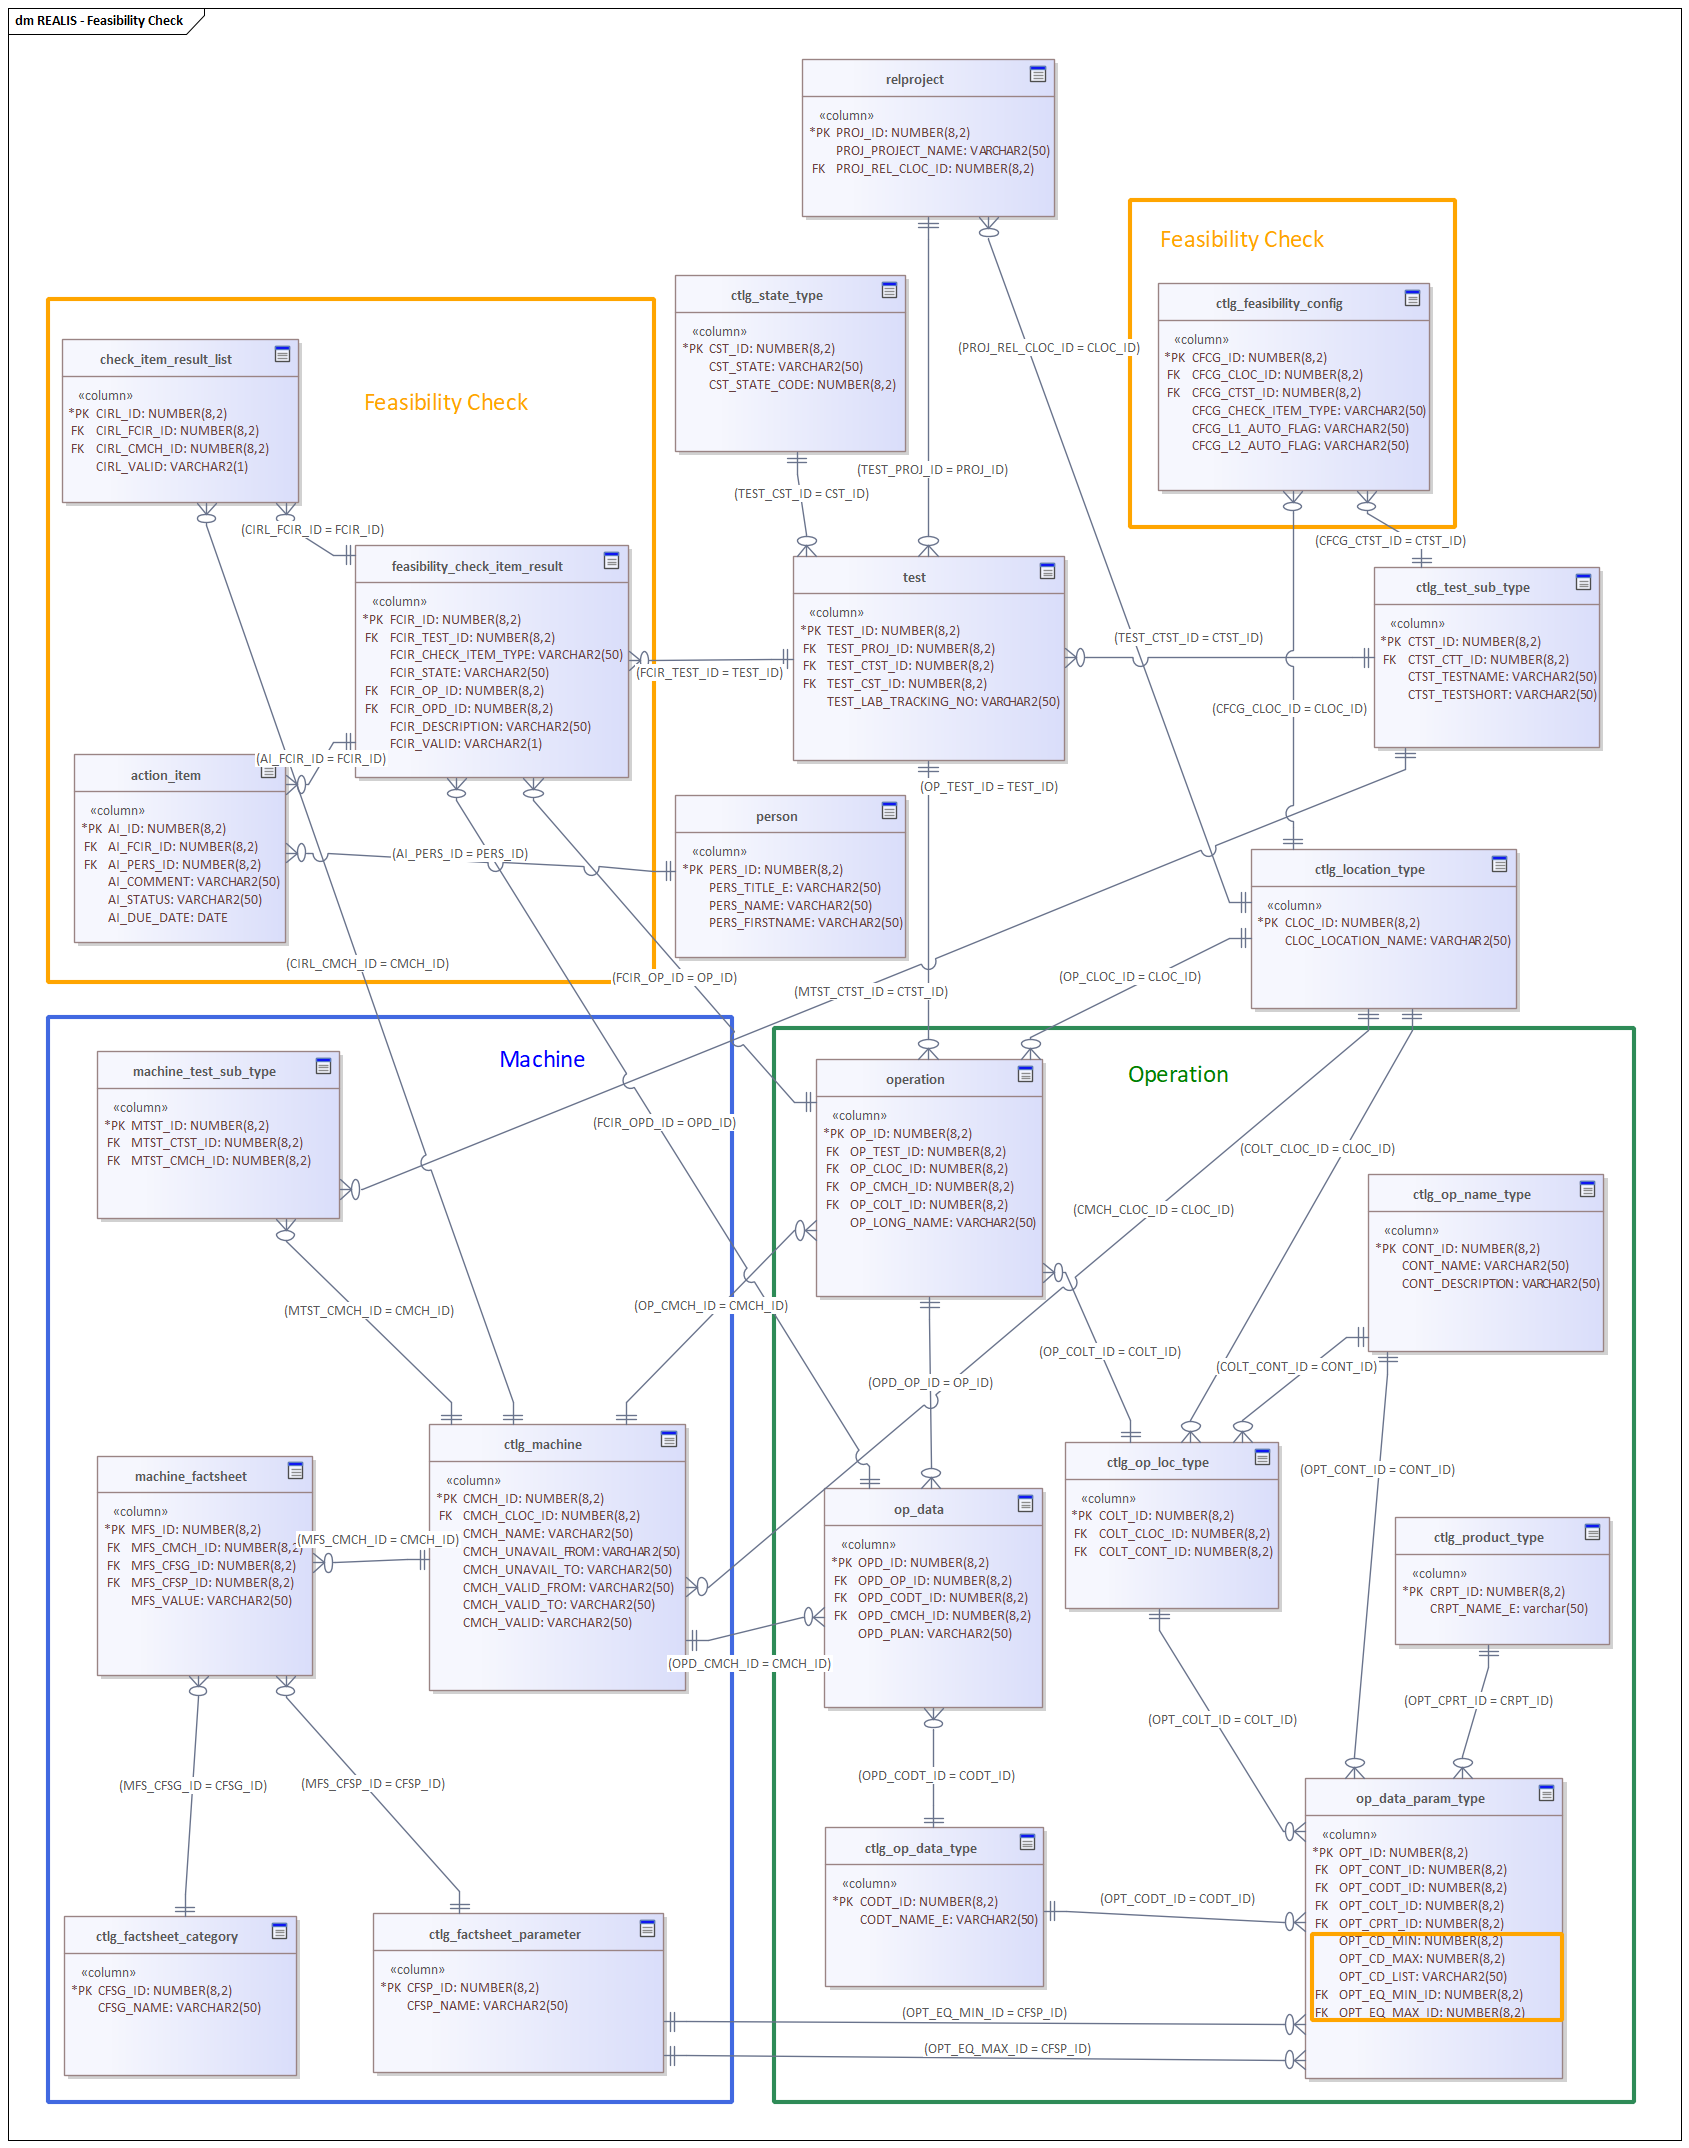
\includegraphics[width=0.98\paperwidth]{bilder/REALIS-Datenbankmodell2.png}}
    \caption{REALIS Datenbankdesign}
    \label{fig:realis-datenbankdesign}
\end{figure}

Die Tabelle \texttt{op\_name\_name\_type} bestimmt welche Arten von Operationen es gibt, und legt indirekt über die Tabelle \texttt{ctlg\_op\_loc\_type} fest, welche Operations-Typen auf welchen Standort verfügbar sind. Darüber hinaus definiert die 
\texttt{op\_data\_param\_type} Tabelle, welcher Parameter bei welcher Operation auf welchem Standort für welchen Produkttypen (\texttt{ctlg\_product\_type}) verfügbar ist. Hierbei sind der Standort und der Produkttyp aber nur optionale Einträge, um generische, standortübergreifende und/oder produktübergreifende Einträge zu realisieren.

Jeder (Stress-)Parameter einer Operation, der einen konkreten Wert definiert (\texttt{OPD\_PLAN}) muss von einer Maschine \texttt{ctlg\_machine} umgesetzt werden (können). Die eng mit der Maschine verknüpften Tabellen, befinden sich in der Abbildung \ref{fig:realis-datenbankdesign} im blau umrandeten Bereich. Eine Maschine ist verknüpft mit einem Machinen-Test-Typen (\texttt{machine\_test\_sub\_type}), der die Machine einem Test-Typen zuweist (\texttt{ctlg\_test\_sub\_type}). Außerdem besitzen Maschinen verschiedene ''Factsheets'' (\texttt{machine\_factsheet}) mit einem Parameter (\texttt{ctlg\_factsheet\_parameter}) und einem Wert (\texttt{MFS\_VALUE}). Dieser Wert korrespondiert mit der PlanValue (\texttt{OPD\_PLAN}) des Operations-Parameters. Hierbei gibt es aber (meist) für jeden Operations-Parameter-Typen zwei zugehörige Maschinen-Factsheet-Parameter(-Typen), die angeben, was jeweils das Minimum und das Maximum der Maschine, bei diesem Parameter ist.


\subsection{Datenbankerweiterung mit Feasibility Check}

Für den Feasibility Check muss die Datenbank nun erweitert werden. Hierbei müssen die Parameter und die Logik des Feasibility Checks, die in Kapitel \ref{Subsec:ParameterdestechnischenFeasibilityChecks} beschrieben worden sind, ermöglicht werden. Zusätzlich dazu sollen die in Kapitel \ref{Chap:Anforderungen} besprochenen Anforderungen eingehalten werden.

Für den Feasibility Check soll der Wert des Parameters der (Stress-)Operation, zum einen auf Sinnhaftigkeit (\gls{ConditionCheck}) und zum anderen auf Durchführbarkeit (\gls{EquipmentCheck}) überprüft werden. Dieser Wert entspricht im Datenbankdesign von \gls{REALIS} dem Eintrag \texttt{OPD\_PLAN} in der Tabelle \texttt{op\_data}, die für den Parameter steht.

Damit dieser Wert auf Sinnhaftigkeit überprüft werden kann, werden in der generischen Tabelle \texttt{opd\_data\_param\_type}, die Operationstyp, Parametertyp, Standort und Produkttyp miteinander verknüpft, zwei neue Einträge hinzugefügt. Diese zwei Einträge beinhalten Werte, die den ''sinnvollen'' Bereich festlegen. Der Eintrag \texttt{OPT\_CD\_MIN} legt dabei die untere Grenze des Bereichs fest, also den minimalen möglichen Wert. Und der Eintrag \texttt{OPT\_CD\_MAX} definiert die obere Grenze, also den maximalen Wert.

Ähnlich wird das ganze für die Überprüfung der Durchführbarkeit angelegt. Hierbei wird die generische Tabelle ebenfalls durch zwei neue Einträge für das Minimum (\texttt{OPT\_EQ\_MIN\_ID}) und das Maximum (\texttt{OPT\_EQ\_MAX\_ID}) erweitert. Diese beinhalten aber nicht direkt zwei Werte, sondern sind Referenzen (Fremdschlüssel) auf zwei Maschinen-Parametertypen (\texttt{ctlg\_factsheet\_parameter}), wobei einer der beiden dem ''minimalen'' Parameter und der andere dem ''maximalen'' Parameter entspricht. Die tatsächlichen Werte stehen dann in der verknüpften \texttt{machine\_factsheet} Tabelle, in dem Feld \texttt{MFS\_VALUE}. Dies wird so gelöst, da, wie im vorherigen Kapitel schon beschrieben, für jeden Operations-Parameter-Typen jede Maschine, die diesen Parameter-Typen umsetzten kann, zwei korrespondierende FactSheet-Parameter(-Typen) besitzt, in die in der mit der Maschine verknüpften Machine-Factsheet Tabelle über einen Fremdschlüssel verwiesen wird. Diese zwei Machine-FactSheet(-Typen) beschreiben dabei den minimalen und maximalen ''Typen'', wobei der tatsächliche minimale und maximale Wert, den die Maschine für diesen Typen umsetzten kann, in dem Machine-Factsheet steht.

Zusätzlich soll ermöglicht werden, dass der automatisierte technische Feasibility Check, ausführlich getestet werden kann, bevor er vollständig ausgerollt wird. Hierfür wird eine Konfiguration (\texttt{ctlg\_feasibility\_config}) in die Datenbank eingefügt, die dem Benutzer ermöglicht abhängig vom (Labor-)Standort (\texttt{ctlg\_location\_type}) und dem Testtypen (\texttt{ctlg\_test\_sub\_type}) festzulegen, welche Test schon mit dem neuen automatisierten System überprüft werden sollen, und welche vorerst noch manuell überprüft werden sollen. Dies wird über den Eintrag \texttt{CFCG\_L1\_AUTO\_FLAG} geregelt.
Die Konfiguration definiert auch den spezifischen ''Check'' im Feld \texttt{CFCG\_CHECK\_ITEM\_TYPE} also, entweder den \gls{ConditionCheck} oder den \gls{EquipmentCheck}.

Die Ergebnisse der durchgeführten Feasibility Checks werden ebenfalls abgespeichert in der Tabelle \texttt{feasibility\_check\_item\_result}. Diese ist verknüpft mit dem Test und, falls möglich mit ''tieferen'' Ebenen, wie der Operation und dem Parameter. Diese sind aber nur optional, da es sein kann, dass das Ergebniss des Checks schon bestimmt werden kann, indem nur der Test überprüft wird, oder da auch die Möglichkeit besteht, dass dieser gar keine Operationen und damit auch keine Parameter besitzt.

Das Ergebnis wird, wie die Konfiguration, abhängig vom ''Check'' gespeichert und enthält ein Feld ... in der die Gründe des Ergebnisses des Checks in Textform abspeichert werden. Auch bekommt die Tabelle ein Flag ..., das aussagt, ob das Ergebnis gültig ist, da man den Feasibility Check für einen Test mehrmals durchführen können soll, wobei alte Ergebnisse erhalten werden aber auf ''invalid'' gesetzt werden.

Wird der \gls{EquipmentCheck} durchgeführt und ist dieser positiv ausgefallen, müssen zusätzlich zum Ergebnis, die gefunden Maschinen abspeichert werden, die sich für die geforderten Parameter eignen. Diese werden in der Tabelle \texttt{check\_item\_result\_list} abspeichert und verknüpfen Maschine mit Feasibility Check Ergebniss.

